\scanpage{180}
\unsure{dira|d'un}, par abus de langage, le schéma en groupe d'autom. de l'anneau différentiel
$\tfrac12$-simplicial $\widehat{\mathcal A}_{\mathbb Z*}$ --).
On a un hom de schémas en groupes
\[
 \Delta:\Omega\longrightarrow G_m
\]
et on a d'ailleurs un inverse à droite
\[
 \unsure{\delta|\sigma}:G_m\mathbin{\text{---}}\Omega
\]
($\unsure{\delta|\sigma}(\lambda)=(A,(B_i)_{i\geq1})$ avec $B_i=0\quad\forall i\geq1$,
$A=\lambda X_0$ i.e. $\varphi_1(X_0)=\lambda X_0$, d'où $\varphi_1(X_1)=\lambda X_1$,
$\varphi_0(T)=\lambda T$, $\varphi_n(X_i)=\lambda X_i\quad\forall0\leq i\leq n$.
Ainsi $\Omega$ est \deleted{\unsure{l'est}} un produit $\frac12$ direct
de $G_m$ et d'un groupe qui est (pro-)unipotent fibre par fibre
\figure{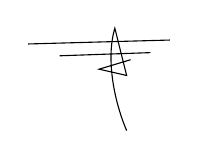
\begin{tikzpicture}
\draw (0,1.1)--(1.8,1.15) (.4,.95)--(1.55,.99);
\draw (1.25,0)..controls(1.1,.35)and(.98,.9)..(1.1,1.3)--(1.25,.7)--(.9,.78)--(1.3,.9);
\end{tikzpicture}}

Si $2$ est inversible\inserted{dans $k$}, \deleted{\unsure{dans}}
\unsure{en plus qu'en est|en plus qu'on est} \unsure{rigueur|vigueur}, tous les autom. de $\widehat{\mathcal A}_{k*}$
respectent le degré extérieur; -- donc
leur effet sur $\operatorname{Hom}(\unsure{X},\widehat{\mathcal A}_{k*})$
\inserted{$\unsure{X}$ ens. $\frac12$-simpl.}
donnent, en passant \unsure{sur la coh.}, des
opérations cohomologiques \uline{ne changeant} pas le \uline{degré} -- i.e. de degré $0$.
Donc \unsure{on ne|si on} trouve rien d'intéressant
-- \unsure{seules les op. évidentes|seules les op. cohom.} (se factorisent par $\Delta$):
\unsure{homo.th.|homoth.} par $\lambda^i$ sur $H^i$ $(\lambda\in k^*)$
\margin{179}
